\documentclass[journal, a4paper]{IEEEtran}
\usepackage[italian]{babel}
\usepackage{booktabs}
\usepackage{siunitx}
\usepackage[utf8]{inputenc}
\usepackage{graphicx} 
\usepackage{url}
\usepackage{amsmath}
\usepackage{amssymb}


\usepackage{keyval}
\usepackage{xcolor}
\usepackage{caption}
\usepackage{subfig}
\usepackage{tikz}
\usepackage{circuitikz}
\usepackage{authblk}
%\usepackage{hyperref}

\begin{document}


% Define document title and author
	\title{Tecnologie Digitali - Logbook Week 11}
	\author[1]{Salvatore Bottaro}
		\author[2]{Lorenzo M. Perrone}
		\affil[1]{\texttt{salvo.bottaro@hotmail.it}}
		\affil[2]{\texttt{lorenzo.perrone.lmp@gmail.com}}
	\markboth{Tecnologie Digitali - Di Lieto}{}
	\maketitle
	
\begin{abstract}
	Logbook di laboratorio di Tecnologie Digitali, a.a. 2015/2016. Week 11.
\end{abstract}

\section{Registri tipo JK}

Nel \emph{flip-flop} di tipo JK è caratterizzato dalla presenza di due ingressi \emph{SET-RESET} che come nel caso del \emph{flip-flop} D prevalgono sullo stato degli altri ingressi. In più sono presenti due ingressi, J e K, anziché uno solo come nel D, che quando sono entrambi nello stato 1 abilitano lo switch delle uscite. Anche in questo caso le uscite vengono modificate solo quando nelle fasi di salita o di discesa del segnale di clock.\\
In figura \ref{fig:pin} è mostrata la zoccolatura del modello studiato in laboratorio, il 14027 della famiglia CMOS, mentre in figura \ref{fig:defpin} sono definiti i vari pin. 

\begin{figure}[htp]
\centering
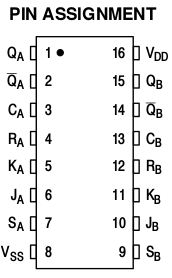
\includegraphics[scale=.4]{pin}
\caption{Zoccolatura del 14027}
\label{fig:pin}
\end{figure}

\begin{figure}[htp]
\centering
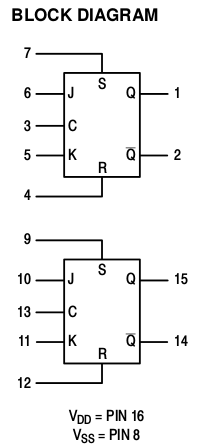
\includegraphics[scale=.4]{scheme}
\caption{Definizione dei pin}
\label{fig:defpin}
\end{figure}

In figura \ref{fig:times} sono definiti i tempi di risposta per gli ingressi J,K e il CLOCK con S e R nello stato 0, mentre in figura \ref{fig:srtimes} sono mostrati i tempi di risposta con S e R variabili.

\begin{figure}[htp]
\centering
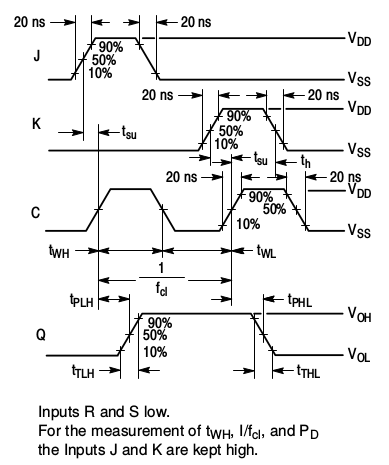
\includegraphics[scale=.4]{times}
\caption{Definizione dei tempi di risposta con S e R bassi}
\label{fig:times}
\end{figure}

\begin{figure}[htp]
\centering
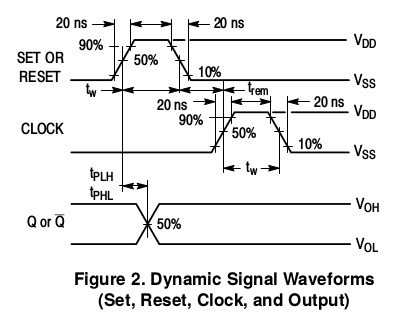
\includegraphics[scale=.4]{srtimes}
\caption{Definizione dei tempi di risposta con S e R variabili}
\label{fig:srtimes}
\end{figure}

In tabella \ref{tab:val} e \ref{tab:data} sono elencati rispettivamente i valori tipici di corrente, alimentazione e consumo e le fasce di tensione del 14027, del tutto identiche a quelle del \emph{flip-flop} D.

\begin{table}[htp]
\centering
\caption{Valori tipici del 14027.}
\label{tab:val}
\begin{tabular}{|c|c|}
\hline 
Grandezza & Valore \\ 
\hline 
Tensione di alimentazione & $V_{min} = -0.5 V$, $V_{max} = 18 V$ \\ 
\hline 
Input current & 10 mA \\ 
\hline 
Consumo massimo & 500 mW \\ 
\hline 
\end{tabular} 
\end{table}

\begin{table}[htp]
\centering
\caption{Fasce di tensione del 14027}
\label{tab:data}
\begin{tabular}{|c|c|c|}
  \hline
  Grandezza & $V_{DD}$ (V)& Valore \\
  \hline
           &  5  &  0.05 V \\ \cline{2-3}
  $V_{OL}$ & 10  &  0.05 V \\ \cline{2-3}
           & 15  &  0.05 V \\ 
  \hline 
           &  5  &  4.95 V \\ \cline{2-3}
  $V_{OH}$ & 10  &  9.95 V \\ \cline{2-3}
           & 15  & 14.95 V \\ 
  \hline \hline
           &  5  &  1.5 V \\ \cline{2-3}
  $V_{IL}$ & 10  &  3.0 V \\ \cline{2-3}
           & 15  &  4.0 V \\ 
  \hline 
           &  5  &  3.5 V \\ \cline{2-3}
  $V_{IH}$ & 10  &  7.0 V \\ \cline{2-3}
           & 15  &   11 V \\ 
  \hline
\end{tabular}
\end{table}

In figura \ref{fig:truth} è mostrata la tavola di verità del JK. Si può notare come per S e R non entrambi nulli e per segnale di clock decrescente le uscite siano identiche al \emph{flip-flop} D; invece per S=R=0 la presenza di un ingresso aggiuntivo comporta delle differene sostanziali, in particolare per la configurazione J=K=1 con clock crescente è previsto lo switch delle uscite.

\begin{figure}[htp]
\centering
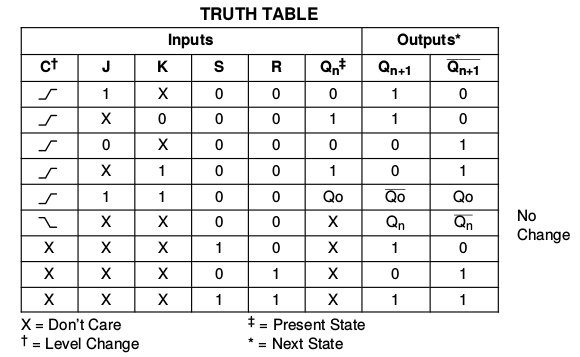
\includegraphics[scale=.4]{truthtable}
\caption{Tavola di varità del \emph{flip-flop} JK}
\label{fig:truth}
\end{figure}

In laboratorio abbiamo verificato che il 14027 impiegato riproducesse la tavola di verità di figura \ref{fig:truth} tramite tester digitale per tutte le combinazioni possibili di S, R, J e K, in particolare abbiamo verificato che per J=K=1 il \emph{flip-flop} si comportasse come un divisore per 2.

\section{Divisore per 3}

Come prima applicazione del \emph{flip-flop} JK abbiamo studiato il divisore per 3 realizzando il circuito in figura \ref{fig:div3}.

\begin{figure}[htp]
\centering
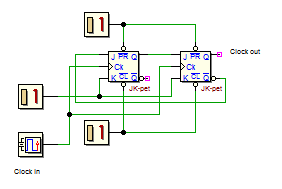
\includegraphics[scale=0.95]{es3}
\caption{Schema del divisore per 3}
\label{fig:div3}
\end{figure}

A partire dalla tavola di verità \ref{fig:truth} è possibile dedurre la sequenza degli stati del circuito, come si vede in tabella \ref{tab:div3}.

\begin{table}[htp]
\centering
\caption{Sequenza degli stati per il divisore}
\label{tab:div3}
\begin{tabular}{|c|c|c|c|}
\hline 
J1 & Q1 & Q2 & Clock \\ 
\hline 
1 & 0 & 1 & $\uparrow$ \\ 
\hline 
0 & 0 & 1 & $\downarrow$ \\ 
\hline 
0 & 0 & 0 & $\uparrow$ \\ 
\hline 
1 & 0 & 0 & $\downarrow$ \\ 
\hline 
1 & 1 & 0 & $\uparrow$ \\ 
\hline 
1 & 1 & 0 & $\downarrow$ \\ 
\hline 
1 & 0 & 1 & $\uparrow$ \\ 
\hline 
\end{tabular} 
\end{table}

Come si nota la prima e l'ultima riga coincidono, per cui si ottiene un ciclo. Il periodo è tre volte quello di clock, per cui a livello di tavola di verità il circuito si comporta come un divisore per 3 e ci si aspetta un duty cycle di $1/3$. Sempre dalla tabella \ref{tab:div3} si vede come lo  stato in cui Q1 = Q2 = 1 non si realizza mai, per cui esso rappresenta uno stato non utilizzato. Inoltre è evidente che non esistono stati non raggiungibili, infatti il circuito possiede due gradi di libertà iniziali, ovvero due ingressi che possono essere settati liberamente, e che possono essere rappresentati da J1 e Q1. Pertanto esistono 4 stati iniziali corrispondenti alle coppie (1,1), (0,0), (1,0), (0,1), di cui i primi 3 effettivamente si riscontrano, mentre l'ultimo sparisce quando il clock si trova nello ''stato'' up, in quanto Q1 assume valore 0 facendo entrare lo stato del circuito dentro il ciclo. L'evoluzione del circuito si può rappresentare graficamente come in figura \ref{fig:graph}, in cui si vede come lo stato (1,1) non compare all'interno del ciclo, rimnendo quindi non utilizzato.\\

\begin{figure}[htp]
\centering
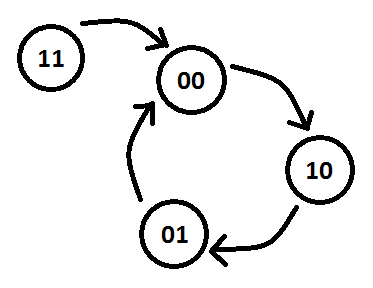
\includegraphics[scale=.5]{Immagine}
\caption{Stati in uscita dal divisore per 3}
\label{fig:graph}
\end{figure}

Abbiamo realizzato effettivamente il circuito collegando l'ingresso del clock al \emph{digital output} 47 e impiegando il VI \texttt{Digital$\_$out4} per generare il segnale, abbiamo collegato le uscite Q1 e Q2 al tester digitale a abbiamo verificato che effettivamente il circuito riproducesse la sequenza di stati previsti.\\
Abbiamo studiato la risposta del circuito collegandolo al generatore di funioni ATTEN, impostando come frequenza di clock 3 kHz. Abbiamo impiegato il fedele VI \texttt{ACQUIS$\_$BASE$\_$2015} e in figura \ref{fig:vi} si può vedere l'esito della misura. Come si può notare il circuito si comporta ancora come divisore per 3 e anche il valore del duty cycle è quello ottenuto precedentemente.

\begin{figure}[htp]
\centering
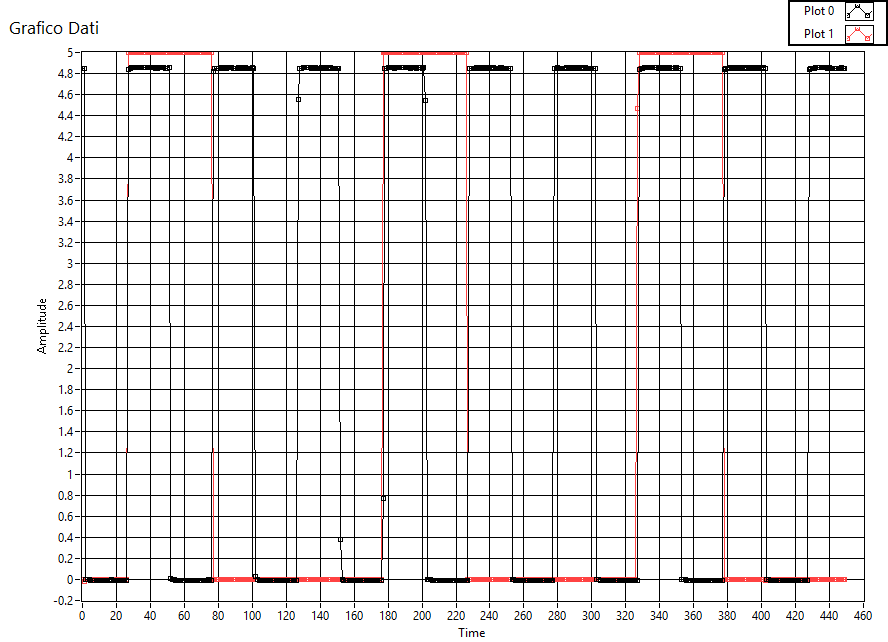
\includegraphics[scale=.25]{es7_sym}
\caption{Confronto fra il segnale di clock (nero) e l'uscita del divisore (rosso)}
\label{fig:vi}
\end{figure}

Per verificare quantitativamente le precedenti affermazioni abbiamo impiegato i VI \texttt{Contatore$\_$freq} e \texttt{Contatore$\_$pulsew}. Tramite il primo VI abbiamo effettuato le misure dei periodi/frequenze dei segnali in ingresso e in uscita, mentre con il secondo VI abbiamo misurato il duty cycle del segnale in uscita al divisore, in entrambi i casi considerando una popolazione statistica di 100 campioni. In tabella \ref{tab:es6-1} e \ref{tab:es6-2} sono mostrati i risultati relativi alle misure di frequenza in ingresso e in uscita, rispettivamente compatibili con i valori impostati e attesi di 3 kHz e 1 kHz. In tabella \ref{tab:es6-3} è mostrata la durata dello stato 1 sul segnale in uscita che è compatibile con $1/3$ del periodo misurato in tabella \ref{tab:es6-2}, per cui il duty cycle del segnale in uscita dal nostro divisore è quello previsto.

\begin{table}[htp]
\centering
\caption{Frequenze e periodi dei segnali in ingresso}
\label{tab:es6-1}
\begin{tabular}{|c|c|c|}
\hline
Grandezza & Valore & Campioni\\
\hline 
Frequenza & 2999.86 Hz & 72 \\ \cline{2-3}
          & 3000.29 Hz & 28 \\ 
\hline 
Periodo & 0.333301 ms & 27 \\ \cline{2-3}
        & 0.333349 ms & 73 \\ 
\hline 
\end{tabular} 
\end{table}

\begin{table}[htp]
\centering
\caption{Frequenze e periodi dei segnali in uscita}
\label{tab:es6-2}
\begin{tabular}{|c|c|c|}
\hline
Grandezza & Valore & Campioni\\
\hline 
Frequenza & 999.951 Hz & 23 \\ \cline{2-3}
          & 999.999 Hz & 77 \\ 
\hline 
Periodo & 1 ms & 80       \\ \cline{2-3}
        & 1.00005 ms & 20 \\ 
\hline 
\end{tabular} 
\end{table}

\begin{table}[htp]
\centering
\caption{Misura duty cycle}
\label{tab:es6-3}
\begin{tabular}{|c|c|c|}
\hline
Tempo  & 0.333351 ms & 64 \\ \cline{2-3}
       & 0.333399 ms & 36 \\ 
\hline 
\end{tabular} 
\end{table}

Ovviamente non è possibile variare il segnale di clock per ottenere un segnale in uscita dal divisore con duty $1/2$ dal momento che ciò che determina la variazione dello stato del circuito è il cambiamento dello stato del clock e non la sua permanenza in uno stato 0 o 1.

\subsection{Hm.1}

\section{Esercizi Vari}

\subsection{Hm.4}
Si consideri il circuito in figura \ref{fig:div5}. Calcolando la tavola di verità è possibile intuire che si tratta di un divisore per 5 con duty cycle $2/5$, come si vede in tabella \ref{tab:div5}. La tabella è stata ottenuta prendendo come stato iniziale la terna (J1, K1, Q1) = (1,1,1), dal momento che tenendo conto del numero di ingressi e uscite e delle loro relazioni il circuito presenta 3 gradi di libertà.

\begin{figure}[htp]
\centering
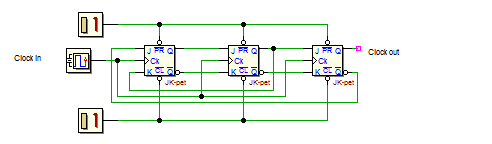
\includegraphics[scale=.8]{hm4}
\caption{Schema divisore per 5}
\label{fig:div5}
\end{figure}

\begin{table}[htp]
\centering
\caption{Tavola del divisore per 5}
\label{tab:div5}
\begin{tabular}{|c|c|c|c|c|c|c|c|c|c|}
\hline
J1 & K1 & Q1 & J2 & K2 & Q2 & J3 & K3 & Q3 & Clock \\ 
\hline 
1 & 1 & 1 & 1 & 0 & 1 & 1 & 0 & 0 & $\uparrow$ \\ 
\hline 
0 & 1 & 0 & 0 & 1 & 1 & 1 & 0 & 1 & $\downarrow$ \\ 
\hline 
0 & 1 & 0 & 0 & 1 & 1 & 1 & 0 & 1 & $\uparrow$ \\ 
\hline 
0 & 0 & 0 & 0 & 1 & 0 & 0 & 1 & 1 & $\downarrow$ \\ 
\hline
0 & 0 & 0 & 0 & 1 & 0 & 0 & 1 & 1 & $\uparrow$ \\ 
\hline 
1 & 0 & 0 & 0 & 1 & 0 & 0 & 1 & 0 & $\downarrow$ \\ 
\hline
1 & 0 & 0 & 0 & 1 & 0 & 0 & 1 & 0 & $\uparrow$ \\ 
\hline 
1 & 0 & 1 & 1 & 0 & 0 & 0 & 1 & 0 & $\downarrow$ \\ 
\hline 
1 & 0 & 1 & 1 & 0 & 0 & 0 & 1 & 0 & $\uparrow$ \\ 
\hline 
1 & 1 & 1 & 1 & 0 & 1 & 1 & 0 & 0 & $\downarrow$ \\ 
\hline
1 & 1 & 1 & 1 & 0 & 1 & 1 & 0 & 0 & $\uparrow$ \\ 
\hline 
0 & 1 & 0 & 0 & 1 & 1 & 1 & 0 & 1 & $\downarrow$ \\ 
\hline 
\end{tabular} 
\end{table}

Sempre dalla tabella si vede che durante il ciclo compaiono 5 degli 8 stati (J1, K1, Q1) possibili, pertanto gli eventuali stati irraggiungibili o inutilizzati vanno da ricercarsi nei 3 assenti. Calcolando la tavola di verità si verifica che sono tutti stati inutilizzati.

\subsection{Hm. 5}

Si consideri il circuito in figura \ref{fig:count3}. Come si evince simulandolo con deeds o calcolandone la tavola di verità (tabella) esso rappresenta un contatore a 3 bit. Essendo un circuito con 3 gradi di libertà e dal momento che le uscite possibili sono 8, tanti quanti i possibili stati iniziali, non ci saranno stati irraggiungibili o inutilizzati.

\begin{figure}[htp]
\centering
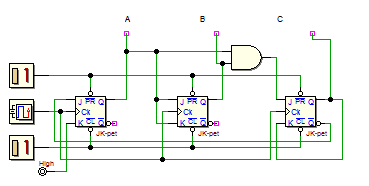
\includegraphics[scale=.8]{hm5}
\caption{Schema contatore a 3 bit}
\label{fig:count3}
\end{figure}

\begin{table}[htp]
\centering
\caption{Tavola del contatore per 3}
\label{tab:count3}
\begin{tabular}{|c|c|c|c|c|c|c|c|c|c|}
\hline
J1 & K1 & J2 & K2 & J3 & K3 & Q3 & Q2 & Q1 & Clock \\ 
\hline 
1 & 1 & 1 & 1 & 0 & 0 & 0 & 0 & 1 & $\downarrow$ \\ 
\hline 
1 & 1 & 1 & 1 & 0 & 0 & 0 & 0 & 1 & $\uparrow$ \\ 
\hline 
1 & 1 & 0 & 0 & 0 & 0 & 0 & 1 & 0 & $\downarrow$ \\ 
\hline 
1 & 1 & 0 & 0 & 0 & 0 & 0 & 1 & 0 & $\uparrow$ \\ 
\hline
1 & 1 & 1 & 1 & 1 & 0 & 0 & 1 & 1 & $\downarrow$ \\ 
\hline 
1 & 1 & 1 & 1 & 1 & 0 & 0 & 1 & 1 & $\uparrow$ \\ 
\hline
0 & 1 & 0 & 0 & 0 & 1 & 1 & 0 & 0 & $\downarrow$ \\ 
\hline 
0 & 1 & 0 & 0 & 0 & 1 & 1 & 0 & 0 & $\uparrow$ \\ 
\hline 
1 & 1 & 0 & 0 & 0 & 0 & 0 & 0 & 0 & $\downarrow$ \\ 
\hline 
1 & 1 & 0 & 0 & 0 & 0 & 0 & 0 & 0 & $\uparrow$ \\ 
\hline
\end{tabular} 
\end{table}

La disposizione delle uscite è scelta per rendere più evidente il comportamento del circuito come contatore per 3.

\subsection{Hm.6}

Si consideri il circuito in figura \ref{fig:contcazzodicane}. Se si legge la sequenza degli stati dalla tavola di verità in tabella \ref{tab:countcazzodicane}, si ha che il circuito fornisce come output la sequenza, in binario, (0,1,2,5,6). Quindi non tutti gli stati entrano nel ciclo del circuito. Infatti calcolando la tavola di verità per gli stati (Q3, Q2, Q1) corrispondenti a 3, 4 e 7 si ottiene che i primi due sono stati irraggiungibili, mentre il terzo è inutilizzato. Si è usato per la tavola di verità lo stesso ordine del caso precedente.

\begin{figure}[htp]
\centering
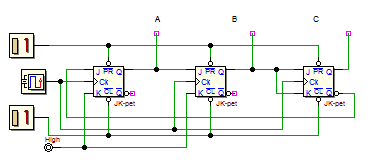
\includegraphics[scale=.8]{hm6}
\caption{Schema del ''contatore a salti''}
\label{fig:contcazzodicane}
\end{figure}

\begin{table}[htp]
\centering
\caption{Tavola del ''contatore a salti''}
\label{tab:countcazzodicane}
\begin{tabular}{|c|c|c|c|c|c|c|c|c|c|}
\hline
J1 & K1 & J2 & K2 & J3 & K3 & Q3 & Q2 & Q1 & Clock \\ 
\hline 
1 & 1 & 1 & 1 & 0 & 0 & 0 & 0 & 1 & $\downarrow$ \\ 
\hline 
1 & 1 & 1 & 1 & 0 & 0 & 0 & 0 & 1 & $\uparrow$ \\ 
\hline 
1 & 1 & 0 & 1 & 1 & 1 & 0 & 1 & 0 & $\downarrow$ \\ 
\hline 
1 & 1 & 0 & 1 & 1 & 1 & 0 & 1 & 0 & $\uparrow$ \\ 
\hline
0 & 1 & 1 & 1 & 0 & 0 & 1 & 0 & 1 & $\downarrow$ \\ 
\hline 
0 & 1 & 1 & 1 & 0 & 0 & 1 & 0 & 1 & $\uparrow$ \\ 
\hline
0 & 1 & 0 & 1 & 1 & 1 & 1 & 1 & 0 & $\downarrow$ \\ 
\hline 
0 & 1 & 0 & 1 & 1 & 1 & 1 & 1 & 0 & $\uparrow$ \\ 
\hline 
1 & 1 & 0 & 1 & 0 & 0 & 0 & 0 & 0 & $\downarrow$ \\ 
\hline 
1 & 1 & 0 & 1 & 0 & 0 & 0 & 0 & 0 & $\uparrow$ \\ 
\hline
1 & 1 & 1 & 1 & 0 & 0 & 0 & 0 & 1 & $\downarrow$ \\ 
\hline
\end{tabular} 
\end{table}

\subsection{Hm. 8}

SI consideri il circuito in figura \ref{fig:count4}. Esso possiede 4 gradi di libertàe quindi ammette 16 possibili stati iniziali del tipo (Q1,Q2,Q3,Q4). In tabella \ref{tab:count4} è mostrata la tavola di verità, in cui compaino solo i J e gli stati uscenti dal clock $\uparrow$. Come si vede il circuito si comporta come un contatore a 4 bit ed esplora tutti e 16 i possibili stati. Pertanto non si hanno stati irraggiungibili o inutilizzati.

\begin{figure}[htp]
\centering
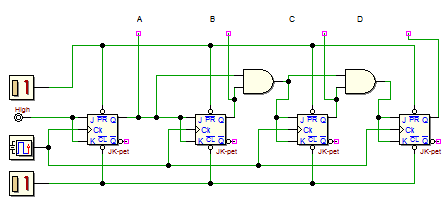
\includegraphics[scale=.8]{hm8}
\caption{Schema contatore a 4 bit}
\label{fig:count4}
\end{figure}

\begin{table}
\centering
\caption{Tavola del contatore 4 bit}
\label{tab:count4}
\begin{tabular}{|c|c|c|c|c|c|c|c|}
\hline 
J1 & J2 & J3 & J4 & Q4 & Q3 & Q2 & Q1 \\ 
\hline 
1 & 1 & 0 & 0 & 0 & 0 & 0 & 1 \\ 
\hline 
1 & 0 & 0 & 0 & 0 & 0 & 1 & 0 \\ 
\hline 
1 & 1 & 1 & 0 & 0 & 0 & 1 & 1 \\ 
\hline 
1 & 0 & 0 & 0 & 0 & 1 & 0 & 0 \\ 
\hline 
1 & 1 & 0 & 0 & 0 & 1 & 0 & 1 \\ 
\hline 
1 & 0 & 1 & 0 & 0 & 1 & 1 & 0 \\ 
\hline 
1 & 1 & 0 & 1 & 0 & 1 & 1 & 1 \\ 
\hline 
1 & 0 & 0 & 0 & 1 & 0 & 0 & 0 \\ 
\hline 
1 & 1 & 1 & 0 & 1 & 0 & 0 & 1 \\ 
\hline 
1 & 0 & 0 & 0 & 1 & 0 & 1 & 0 \\ 
\hline 
1 & 1 & 0 & 0 & 1 & 0 & 1 & 1 \\ 
\hline 
1 & 0 & 1 & 0 & 1 & 1 & 0 & 0 \\ 
\hline 
1 & 1 & 0 & 0 & 1 & 1 & 0 & 1 \\ 
\hline 
1 & 0 & 0 & 0 & 1 & 1 & 1 & 0 \\ 
\hline 
1 & 1 & 1 & 1 & 1 & 1 & 1 & 0 \\ 
\hline 
1 & 0 & 0 & 0 & 0 & 0 & 0 & 0 \\ 
\hline 
\end{tabular}
\end{table}

\end{document}